\chapter{Graph Machine Learning}
\label{chp: background}

% \addcontentsline{toc}{chapter}{Graph Machine Learning}

This chapter will present the main scientific background required for this work, mainly from network science and graph machine learning.

\section{Graph theory \& Network science}
The field of \emph{network science} studies methods for analysing specific properties of graph-structured data in order to obtain insight that might be useful for building a predictive model of the target graph/network. Scientific background is mainly drawn from graph theory from mathematics, statistical mechanics from physics, and data mining from computer science. Certain graph-related concepts from this branch of science proved extremely useful for this work, and as such, their main ideas and definitions will be presented in the following sections.

\subsection{Graph fundamentals}
\begin{definition}
A \emph{finite graph} $G$ is defined as the ordered pair of two finite sets, $G=(V,E)$ where:
\begin{itemize}
\item $V=\{v_1, \dots, v_N\}$ is a finite set of elements, which are referred to as \emph{nodes} (or \emph{vertices}, \emph{points} etc.);
\item $E$ is a set of elements referred to as \emph{edges} (or \emph{links}, \emph{lines} etc.), where an edge is defined as an ordered pair of nodes: $E=\{(v_i,v_j)|v_i,v_j \in V\}$.
\end{itemize}
\end{definition}
For the purpose of this text, we will accept the terms \emph{graph} and \emph{network} to be equivalent, even though in some contexts, this might not be the case.

\begin{definition}
Graphs can be of two main types: \emph{directed} or \emph{undirected}.
\begin{itemize}
\item \emph{Undirected} graphs have the property that edges are symmetric w.r.t. the pair of nodes, i.e. the following holds: $\forall v_i,v_j \in V, (v_i,v_j) \in E \Rightarrow (v_j, v_i) \in E$;
\item \emph{Directed} graphs have the property that edges can have a meaningful direction, i.e. $\exists v_i,v_j \in V, (v_i,v_j) \in E \wedge (v_j, v_i) \not\in E$.
\end{itemize}
\end{definition}

\begin{definition}
The \emph{adjacency matrix} of a graph $G=(V, E)$ is defined as the matrix $A \in \{0,1\}^{|V| \times |V|}$, whose elements are computed as follows:
\begin{equation}
\forall i,j \in \{1, \dots, |V|\}, A_{ij} = \begin{cases}1 &\text{, if }(v_i, v_j) \in E \\ 0 & \text{, otherwise} \end{cases}
\end{equation}
\end{definition}

\begin{definition}
Given a graph $G=(V, E)$, the \emph{degree} of a node $v \in V$ is defined as the number of edges the node participates in: 
\begin{equation}
d(v) = |\{u|u \in V, (v, u) \in E \vee (u, v) \in E \}|
\end{equation}

For directed graphs, due to the asymmetry of edges, the separate notions of \emph{out-degree} and \emph{in-degree} can be defined:
\begin{itemize}
\item $d_{\text{out}}(v) = |\{u|u \in V, (v, u) \in E \}|$;
\item $d_{\text{in}}(v) = |\{u|u \in V, (u, v) \in E \}|$.
\end{itemize}
\end{definition}

\begin{definition}
Given a graph $G=(V, E)$, the \emph{neighbourhood} of a node $v \in V$ is the defined as the set of nodes $v$ is directly connected to with an edge: \begin{equation}
N(v)=\{u|u\in V, (v,u) \in E \vee (u,v) \in E \}
\end{equation} 
Analogously as for node degree, the notions of \emph{in-neighbourhood} and \emph{out-neighbourhood} can be defined. Observe that $d(v)=|N(v)|$.
\end{definition}

\begin{definition}
A \emph{path} in a graph $G=(V, E)$ is a sequence of nodes $v_1,\dots,v_n \in V$ in which every pair of consecutive nodes are connected by an edge:\\ $\forall i \in \{1,\dots,n-1\},(v_i,v_{i+1})\in E$. A \emph{cycle} is a path where $v_1=v_n$.
\end{definition}

\begin{definition}
Given a graph $G=(V, E)$ and a subset of the nodes $V' \subseteq V$, a \emph{subgraph} $G'=(V', E')$ is obtained by considering the edges only between the nodes in the subset: $E' = \{(v, u)|(v, u) \in E, v,u \in V'\}$.
\end{definition}

\begin{definition}
Between a pair of nodes in a graph, there might be more than one or no paths, depending on the connectivity. If there are multiple paths between the pair, the ones with the minimum length are called \emph{shortest paths}.
\end{definition}

\begin{definition}
A directed graph is \emph{strongly connected} if a path exists between all pairs of nodes in the graph. A directed graph is \emph{weakly connected} if a path exists between all pairs of nodes in the undirected graph obtained by converting all of the edges of the original directed graph in undirected form. If a whole directed graph is not strongly/weekly connected, but a subgraph is, this subgraph is called a \emph{strongly/weakly connected component} of the original graph, respectively.
\end{definition}

\subsection{Importance measures}

Network science teaches that networks have specific relevant computable attributes that can be used to analyze the network in order to summarize, characterize, and model it. One class of these metrics deals with the problem of how to assign an \enquote{importance} score to nodes and edges, but different metrics encode different contexts in doing this.

For example, there exist several so-called \emph{centrality} indices that attempt to rank nodes or edges for different purposes, such as \emph{degree centrality}, \emph{betweenness centrality}, \emph{closeness centrality}, etc. Generally, these metrics give more importance to nodes/edges, which contribute more to the graph's connectivity and are derived from the node degree, number of paths, or other elementary properties.

\begin{definition}
The \emph{betweenness centrality} of an edge is defined as the number of shortest paths in the graph that pass through (contain) that edge in ratio with the total number of shortest paths.
\end{definition}

The clustering coefficient scores vertices on the number of connections present in their neighbourhood in ratio with the number of total possible. This measure is essential when comparing networks w.r.t. average local connectivity and gauging a rich community structure.

\begin{definition}
Given a graph $G=(V, E)$, the \emph{clustering coefficient} $cc(v)$ is computed as: \begin{equation}
cc(v)=\frac{|E'(v)|}{{|N(v)| \choose 2}} = \frac{2|E'(v)|}{|N(v)|(|N(v)|-1)},\end{equation}
where $|E'(v)|$ is the number of edges in the subgraph $G'(v)=(N(v), E'(v))$ formed out of the neighbourhood of $v$, $N(v)$.
\end{definition}

More intricate algorithms for computing node importance in network science historically were devised by viewing the problem as a form of \enquote{edge flow}: for example, the flow of current in the context of physics or in the context of page ranking on the World Wide Web, traffic through hyperlinks. These algorithms have in common the idea that nodes start with an equal \enquote{amount of importance} in regards to some context, but this importance can continuously flow through the edges of the network. Depending on the network connectivity, in the end, the process will converge to some steady state, where each node has the correct amount of true importance. We will elaborate on two such well-established algorithms in computer science that were considered for this work.

\paragraph{HITS} In 1999 \cite{kleinberg_authoritative_1999} described the Hyperlink-Induced Topic Search (HITS) algorithm for rating Web pages. The idea behind HITS stemmed from insight into creating web pages when the Internet was initially forming. The author defined two notions: a good \emph{hub} represents a page that points to many other pages, while a good \emph{authority} represents a page that is linked by many different hubs. By modelling the pages as nodes and the possible hyperlinks between them as edges, one can use the hubs and authorities scheme to construct an algorithm for computing two importance measures for the graph nodes: hub and authority values. Implementation-independent pseudocode for the process is given in Algorithm \ref{algorithm:hits}.

\begin{algorithm}[H]
\caption{Hubs and authorities}
\label{algorithm:hits}
\begin{algorithmic}
\STATE{\textbf{input} graph $G = (V, E)$}
\STATE{\textbf{initialize} $\forall v \in V, \pmb{h}_0(v) = \pmb{a}_0(v) = \frac{1}{|V|^2}$}
\WHILE{convergence criteria not reached}
\STATE{\textbf{update} $\forall v \in V, \pmb{h}_{t}(v) = \sum_{u \in N_{\text{out}}(v)}{\pmb{a}_{t-1}(u)}$}
\STATE{\textbf{update} $\forall v \in V, \pmb{a}_{t}(v) = \sum_{u \in N_{\text{in}}(v)}{\pmb{h}_{t-1}(u)}$}
\STATE{\textbf{normalize} $\forall v \in V, \pmb{h}_t(v) = \frac{\pmb{h}_t(v)}{||\pmb{h}_t||_2}, \pmb{a}_t(v) = \frac{\pmb{a}_t(v)}{||\pmb{a}_t||_2}$}
\ENDWHILE
\RETURN{final hub scores $\pmb{h} \in \mathbb{R}^{|V|}$, final authority scores $\pmb{a} \in \mathbb{R}^{|V|}$}
\end{algorithmic}
\end{algorithm}

\paragraph{PageRank} Brin and Page published in \cite{brin_anatomy_1998} how their novel search engine works. They describe the PageRank algorithm for ranking Web pages, a technique for obtaining node importances extremely widespread in use even today. The underlying assumption employed by PageRank is that more important websites/nodes are likely to receive more links/edges from other important websites/nodes. Expressly, PageRank scores for nodes represent probabilities that a random walker (Web crawler) will end up at the nodes while also considering that this walker can teleport to a random node when reaching a dead end. Implementation-independent pseudocode for the process is given in Algorithm \ref{algorithm:pagerank}.

\begin{algorithm}[H]
\caption{PageRank}
\label{algorithm:pagerank}
\begin{algorithmic}
\STATE{\textbf{input} adjacency matrix $A \in \mathbb{R}^{|V| \times |V|}$, teleportation probability $p \in [0,1]$}
\STATE{\textbf{compute} $\forall i,j \in \{1,\dots,|V|\}, R_{ij} = \frac{A_{ji}}{\sum_{k=1}^{|V|}{A_{jk}}}$}
\STATE{\textbf{compute} $M = (1-p)R + p \frac{1}{|V|}$}
\STATE{\textbf{compute} $\pmb{r}$, eigenvector of $M$ associated to the largest eigenvalue}
\RETURN{PageRank scores $\pmb{r} \in \mathbb{R}^{|V|}$}
\end{algorithmic}
\end{algorithm}

\subsection{Community structure}
Network science also focuses on analysing another common and important characteristic of graphs: community structure. In the context of networks, community structure details groups of nodes more densely connected internally than to other nodes. This inhomogeneity of connections would suggest that the network has certain natural divisions within it.

\emph{Communities} are classically defined as a disjoint partition of the node set; however, in some contexts, allowing overlapping communities can also be relevant.
\begin{definition}
Given a graph with a set of nodes $V$, \emph{communities} are node sets $C_1, \dots, C_K$ that form a \emph{covering} of $V$: $C_1, \dots, C_K \subseteq V$, $\bigcup_{j=1}^{K}{C_j} = V$. In the more common \emph{disjoint} case, the communities form a disjoint partitioning of $V$: $\bigcap_{j=1}^{K}{C_j}=\emptyset$. However, this is not true in general, where \emph{overlapping regions} might exist between communities: $\exists j,k \in \{1,\dots,K\}$, $j \neq k$, such that $O_{j,k} = C_j \cap C_k \neq \emptyset$.
\end{definition} 

For the models presented in this thesis, finding an underlying community structure in the input network is vital for several reasons. Communities allow our model to create a large-scale map of the network, as individual communities can be viewed as meta-nodes linked with meta-edges according to the inter-community connectivity of the data. In addition, in real-world networks, such as the Swisscom knowledge graph, community structure is often strongly present.

\begin{definition}
    Given a graph $G=(V,E)$ with community sets $C_1, \dots, C_K$, \emph{graph coarsening} involves constructing a new community-level interaction graph according to the node-to-community memberships and original edges. Formally, we output $G^C=(V^C,E^C)$, where $V^C=\{C_1,\dots,C_K\}$ and $E^C=\{(C_k,C_l)|\exists (v,u) \in E,v \in C_k \wedge u \in C_l\}$.
\end{definition}

Communities can have meaning beyond just structural units of the graph and paint a clearer picture of the system. However, the most crucial point is that communities can often have very different properties than the average properties of the networks, so models that take these local deviations into account should be more robust. Community detection and graph coarsening are the two key processes that allow us to employ both holistic and reductionist views and models of graph data.


% \subsection{Random walks}
% In the context of graphs, a random walk is a path through the graph for which the sequence of nodes has been obtained by random sampling from a distribution over the set of nodes. Initially, the starting node is sampled from the full node-set, while successive nodes are obtained by sampling the neighbourhood of the current node but independently of past nodes.

% \begin{definition}
% Given a graph $G = (V, E)$, a \emph{random walk} of length $L$ is a realisation of a discrete stochastic process $\{V_i\}_{i=1}^L$ where $V_1$ is a random variable with support $V$ and probability mass function $\lambda$, $\sum_{v \in V}{\lambda(v)}=1$, while $\forall t\in \{2,\dots,L\}$, $V_t$ is a random variable with support $N(V_{t-1})$ and probability mass function $\mu_t$, $\sum_{u \in N(V_{t-1})}{\mu_t(u)}=1$.
% \end{definition}

% Sampling random walks from a graph is a way of converting the graph into a set of node sequences, from which much richer information can be extracted, such as multi-hop connections and node-context pairs.
% \begin{definition}
% Given a random walk $W=\{V_i\}_{i=1}^L$, the \emph{context} of a node $V_i \in W$ is the set of nodes that lie within a certain number of hops $\rho$ to the node along the random walk path: $C(V_i, W, \rho)=\{V_j|V_j\in W,1 \leq |i-j| \leq \rho\}$, where $\rho$ is referred to as the \emph{context radius}. The set of \emph{node-context pairs} is thus formed as: 
% \begin{equation}
% \bigcup_{i=1}^{L}{\{(V_i, V_j)|V_i, V_j \in W,V_j \in C(V_i, W, \rho)\}}
% \end{equation} 
% \end{definition}


\section{Machine learning}
Machine learning (ML) is the computer science study of algorithms that build a \emph{model} with \emph{parameters} based on sample \emph{data} in order to make \emph{predictions} or \emph{decisions} without being explicitly programmed to do so. The process of learning the model's parameters is called \emph{training}. Machine learning is seen as a part of the computer science field of artificial intelligence and is closely related to computational statistics, though not all ML models are stochastic. We will present the basic concepts and those related to the neural network type of ML models relevant to this work through the rest of this chapter. 

\subsection{Fundamentals}

\begin{definition}
We define a \emph{model} as the pair $M = (\pmb{\theta}, f)$, where:
\begin{itemize}
\item $\pmb{\theta} \in \Theta$ is referred to as the set of \emph{parameters}, belonging to the \emph{parameter space} $\Theta$;
\item The function $f: \mathcal{X} \times \Theta \to \mathcal{Y}$ accepts values from the \emph{input space} $\mathcal{X}$ and based on the current parameter values produces elements from the \emph{output space} $\mathcal{Y}$.
\end{itemize}
Usually the application of a model is denoted through the shorthand notation:\\ $y = f(\pmb{x}, \pmb{\theta})$, where $\pmb{x} \in \mathcal{X}$, $y \in \mathcal{Y}$.
\end{definition}

Every model with parameters is applied to a set of sampled data.

\begin{definition}
A \emph{datapoint} $\pmb{d}=(\pmb{x}, y)$ is a random sample from the set $\mathcal{D} = \mathcal{X} \times \mathcal{Y}$. In general, the underlying probability distribution over $\mathcal{D}$ of the data source is not known. 

In most cases, the model's input space is $D$-dimensional real ($\mathcal{X}=\mathbb{R}^D$), and the input samples $\pmb{x} \in \mathbb{R}^D$ are referred to as \emph{feature vectors}. At the same time, the output space is often also numeric and one-dimensional, with the output samples $y \in \mathcal{Y}$ called \emph{target values}.  

A \emph{dataset} $\pmb{D}$ is a finite collection of datapoints $\pmb{d}_1,\dots,\pmb{d}_N$.
\end{definition}

In order to evaluate how well a model performs on a task, we define a loss function.

\begin{definition}
For each datapoint $\pmb{d}_i=(\pmb{x}_i, y_i)$ of a dataset, a \emph{loss} function $\mathcal{L}_{i}$, $\mathcal{L}_{i}: \mathcal{Y} \times \mathcal{Y} \to \mathbb{R} $ outputs a numeric value scoring how closely a model $M = (\pmb{\theta}, f)$ represents the output sample $y_i$ as the function of the input sample $\pmb{x}_i$. We will denote the application of the loss function with $\mathcal{L}_{i}(y_i, f(\pmb{x}_i, \pmb{\theta}))$.

We can define the loss function on the level of the whole dataset as the expected per-datapoint loss over the dataset. This expectation cannot be computed as the underlying data distribution is not known, so we use an empirical estimate: \begin{equation}
\mathcal{L}(\pmb{D}, \pmb{\theta}, f) = \frac{1}{N}\sum_{i=1}^{N}{\mathcal{L}_{i}(y_i, f(\pmb{x}_i, \pmb{\theta}))}
\end{equation}
\end{definition}

Before delving further, we will give an example. One of the simplest models we can impose is the \emph{linear model}. Its characteristics are as follows:
\begin{itemize}
\item $\mathcal{X} = \mathbb{R}^D$, $\mathcal{Y}=\mathbb{R}$;
\item $\pmb{\theta} = (\pmb{w}, b)$, where $\pmb{w} \in \mathbb{R}^D$ are referred to as the \emph{weights} and $b \in \mathbb{R}$ is called the \emph{bias} value;
\item $f(\pmb{x}, \pmb{\theta}) = \sum_{j=1}^{D}{w_j x_j} + b$, i.e. the output is modelled as a linear combination of the input;
\item The loss function is most often the so called Mean Squared Error (MSE): \begin{equation}
\mathcal{L}(\pmb{D}, \pmb{\theta}, f) = \frac{1}{2N}\sum_{i=1}^{N}{(y_i - f(\pmb{x}_i, \pmb{\theta}))^2}
\end{equation}
\end{itemize}

The general linear model is an example of a typical model that is said to be able to perform \emph{regression} - prediction of real-valued continuous output. When the output space is a \emph{discrete} set, we refer to that prediction problem as \emph{classification}. Instead of the MSE loss, the cross-entropy loss function is chosen for classification problems.

\begin{definition}
Given a discrete output space $\mathcal{Y}=\{1,\dots,D\}$, we define the \emph{cross-entropy loss} as: $\text{CrossEntropy}: [0, 1]^D \times \mathcal{Y} \to \mathcal{R}$, such that:
\begin{equation}
\forall \hat{\pmb{y}} \in [0, 1]^D, y \in \mathcal{Y}, \text{CrossEntropy}(\hat{\pmb{y}},y)= - \log{\left(\frac{e^{\hat{y}_y}}{\sum_{d=1}^{D}{e^{\hat{y}_d}}}\right)}\end{equation}
\end{definition}

\begin{definition}
Model \emph{training} consists of finding the optimal parameter values $\pmb{\theta}^*$ such that the loss function over the dataset is minimized. Formally the following minimization problem needs to be solved: $\pmb{\theta}^* = \argmin_{\pmb{\theta} \in \Theta}{\mathcal{L}(\pmb{D}, \pmb{\theta}, f)}$.
\end{definition}

However, as the loss function can be arbitrarily complex, in very few scenarios can the minimization problem be analytically solved in exact form. As such, iterative numeric algorithms called \emph{optimizers} are applied. These are based on low-degree local approximations of the loss function to obtain simple update formulas for the parameters. In order to give strict theoretical convergence guarantees, optimization algorithms usually assume that the loss function has particular desirable properties, such as convexity and smoothness.

The starting point for all developed loss optimization algorithms is the Gradient Descent (GD) technique and its probabilistic variant Stochastic Gradient Descent (SGD). These methods rely on a first-order Taylor expansion of the loss. Therefore it is required to compute the gradient (vector of first derivatives) of the loss function w.r.t. the model parameters in every iteration. Pseudocode for GD and SGD is given in Algorithm \ref{algorithm:gd} and \ref{algorithm:sgd}, respectively.

\begin{algorithm}
\caption{Gradient Descent}
\label{algorithm:gd}
\begin{algorithmic}
\STATE{\textbf{input} model function $f$, initial parameter values $\pmb{\theta}_0$, learning rate $\gamma \in \mathbb{R}^{+}$}
\STATE{\textbf{set} $t = 0$}
\WHILE{convergence criteria not reached}
\STATE{\textbf{update} $\pmb{\theta}_{t+1} = \pmb{\theta}_{t} - \gamma \nabla_{\pmb{\theta}}\mathcal{L}(\pmb{D}, \pmb{\theta}_{t}, f)$}
\STATE{\textbf{update} $t = t+1$}
\ENDWHILE
\RETURN final parameter values $\pmb{\theta}_{t}$
\end{algorithmic}
\end{algorithm} 

\begin{algorithm}
\caption{Stochastic Gradient Descent}
\label{algorithm:sgd}
\begin{algorithmic}
\STATE{\textbf{input} model function $f$, initial parameter values $\pmb{\theta}_0$, learning rate $\gamma \in \mathbb{R}^{+}$}
\STATE{\textbf{set} $t = 0$}
\WHILE{convergence criteria not reached}
\STATE{\textbf{sample} $i \in \{1,\dots,N\}$ uniformly at random}
\STATE{\textbf{update} $\pmb{\theta}_{t+1} = \pmb{\theta}_{t} - \gamma \nabla_{\pmb{\theta}}\mathcal{L}_i(y_i, f(\pmb{x}_i, \pmb{\theta}_{t}))$}
\STATE{\textbf{update} $t = t+1$}
\ENDWHILE
\RETURN final parameter values $\pmb{\theta}_{t}$
\end{algorithmic}
\end{algorithm} 


\subsection{Neural networks}
The power of a model to fit any observed data depends on the complexity and generality of its definition, as well as the number of possible parameter values that can be optimized. With the linear model in the example presented above, we can only represent linear dependence relations between observed input and target data. As such, to model a general \emph{non-linear} relation, one introduces a non-linear component to the definition.

In the machine learning theory of Artificial Neural Networks, one builds more complex models starting from the most elementary building block, the artificial neuron.
\begin{definition}
A \emph{neuron} is the model obtained when a non-linear function $\phi$ is applied over a linear model i.e. $\mathcal{X} = \mathbb{R}^D$, $\mathcal{Y}=\mathbb{R}$, $\pmb{\theta} = (\pmb{w}, b)$, $f(\pmb{x}, \pmb{\theta}) = \phi\left(\sum_{j=1}^{D}{w_j x_j} + b\right)$. The function $\phi: \mathbb{R} \to \mathbb{R}$ is called the \emph{activation function}. It should possess some desirable properties (such as boundedness of gradients) in order to obtain certain theoretical guarantees. The most commonly utilized are the functions $\text{ReLU}(x)=\max(0,x)$, $\sigma(x)=\frac{1}{1+e^{-x}}$, $\tanh(x)$ etc. The inputs to the activation function obtained using the linear model are called \emph{activations}.
\end{definition}

\begin{definition}
A neural network \emph{layer} $\ell$ is the model $M = (\pmb{\theta}_{\ell}, f_{\ell})$ for which $\pmb{\theta}_{\ell} = \{\pmb{\theta}_1, \dots, \pmb{\theta}_K\}$ and $f_{\ell}: \mathcal{X} \to \mathcal{Y}^K$ is defined as $f_{\ell}(\pmb{x}, \pmb{\theta}) = [f(\pmb{x}, \pmb{\theta}_1),\dots,f(\pmb{x}, \pmb{\theta}_K)]$, where $M_1=(\pmb{\theta}_1, f),\dots,M_K=(\pmb{\theta}_K, f)$ are the constituting sub-models, each of same type but with possibly different parameters. Note that the layer accepts inputs from the same input space as every sub-model and just collects the outputs from each together.
\end{definition}

The simplest example of a neural network layer is the so-called \emph{fully-connected layer}, which is just a collection of multiple neurons: $\pmb{\theta}=(W, \pmb{b}), f_{\ell}(\pmb{x}, \pmb{\theta}) = \phi\left(W\pmb{x} + \pmb{b}\right)$, where $W \in \mathbb{R}^{K \times D}$ is a matrix whose rows are the weights of each neuron and the vector $\pmb{b} \in \mathbb{R}^K$ contains the bias values.

\begin{definition}
A \emph{neural network} is a model defined as a composition of a finite number of layers: $\pmb{\theta}=\{\pmb{\theta}_{\ell}^{(1)},\dots,\pmb{\theta}_{\ell}^{(L)}\}$ and $f = f_{\ell}^{(1)} \circ \dots \circ f_{\ell}^{(L)}$. Commonly the first layer of a neural network is referred to as the \emph{input layer}, the final one the \emph{output layer} and all layers in between as \emph{hidden layers}. 
\end{definition}

When all neural network layers are fully connected, we call this type of neural network a Multi-Layer Perceptron (MLP). Figure \ref{fig:mlp_example} gives a visual example of a MLP. A surprising fact that can be proven about MLPs is that given that the number of neurons is large enough, an MLP with a single hidden layer can approximate almost all classes of functions with any desired accuracy. This fact, proven by \cite{hornik_multilayer_1989} is referred to as the \enquote{Universal Approximation Theorem}. For this reason, neural networks have seen an understandable amount of popularity in computer science research.

\begin{figure}[H]
\centering
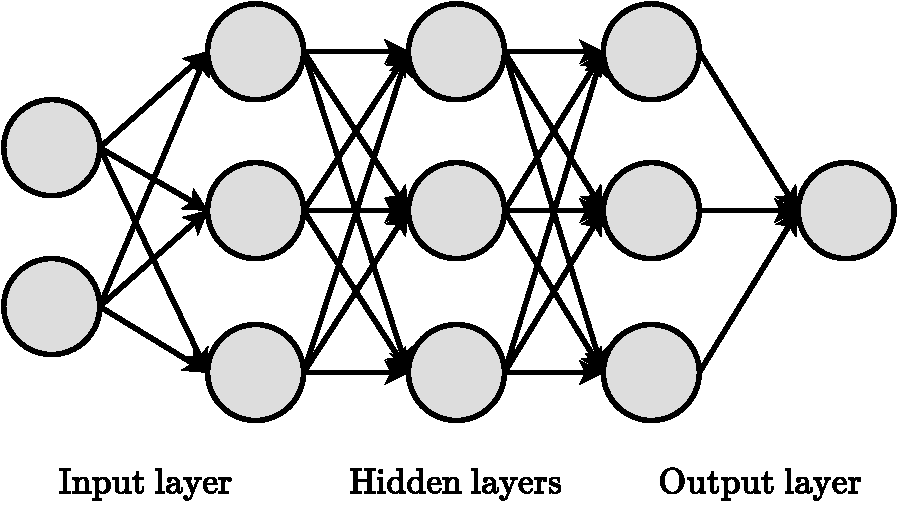
\includegraphics[width=0.5\textwidth]{figures/background/mlp_example}
\caption[Example of a Multi-Layer Perceptron (MLP).]{Example of a Multi-Layer Perceptron (MLP), with two inputs, three hidden layers each made up of three neurons and one output.}
\label{fig:mlp_example}
\end{figure}

However, research by \cite{telgarsky_representation_2015, telgarsky_benefits_2016} and other works have shown that by increasing the number of neurons per layer, we only obtain a linear increase in the representation power of neural networks. However, by adding more layers, the benefits are \emph{exponential}. In the past decade, this has led to a massive explosion of research in the development of \emph{deep} neural network models with multi-layer architectures. The field had been coined \emph{deep learning} accordingly. Results that models with specific combinations of layers with many different structures perform better than the general MLP are frequent insights obtained from this field of research. In the following paragraphs, we will briefly describe the most common types of layers present in models related to and utilized in this work.

\paragraph{Embeddings} \emph{Embedding layers} are used purely to store embedding vectors and function as a simple lookup table. Their input values denote indices of the columns of a matrix in which the embeddings are stored. In order to obtain the embeddings through matrix multiplication, the indices are \emph{one-hot encoded}: $\pmb{\theta}_{\ell} = W \in \mathbb{R}^{D \times N}$, $f_{\ell}: \{1,\dots,N\} \to \mathbb{R}^D$, $\forall x \in \{1,\dots,N\}, f_{\ell}(x, \pmb{\theta}_{\ell}) = W \tilde{\pmb{x}}$, where $\tilde{\pmb{x}} \in \mathbb{R}^N, \tilde{x}_i = \mathbb{I}(i = x)$ is the one-hot encoded input, $D$ is the \emph{embedding dimension} and $N$ is the \emph{input dimension} (number of embeddings to store).

\paragraph{Convolution} Unlike for fully-connected layers, where the whole input is linearly combined with the weights, convolutional layers apply a smaller set of weights, called the \emph{filter} or \emph{kernel}, to each smaller section of the input of equal size, using the \emph{discrete convolution operation} in order to obtain the list of outputs. In this manner the model is more robust to \emph{translations} of the input. The form of this type of layer for one-dimensional input would be: 
\begin{align}
\pmb{\theta}_{\ell} &= (\pmb{w} \in \mathbb{R}^{S}, b \in \mathbb{R}), f_{\ell}: \mathbb{R}^{D} \to \mathbb{R}^{D-S+1}, \nonumber \\
\forall i &\in \{1,\dots,D-S+1\}, y_i = b + \sum_{j=1}^{S}{x_{i+j-1}w_j}    
\end{align}

\paragraph{BatchNorm} \emph{Batch normalization layers} were proposed by \cite{ioffe_batch_2015} in order to control the statistics (mean/variance) of the neural network activations during training and avoiding issues such as parameter gradients decaying to $0$. BatchNorm layers are models that achieve this by learning how to re-normalize their inputs: $\pmb{\theta}_{\ell} = (\gamma, \beta)$, $f_{\ell}(\pmb{x}, \pmb{\theta}_{\ell}) = \gamma \odot \frac{\pmb{x}-\hat{\mu}(\pmb{x})}{\sqrt{\hat{\sigma}^2(\pmb{x}) + \varepsilon}} + \beta$, $\varepsilon << 1$.

\paragraph{Dropout} \emph{Dropout layers} were proposed by \cite{hinton_improving_2012} as a form of regularization for deep neural networks, i.e., they control parameter values in order to avoid the model over-fitting the data. The effect is achieved by randomly selecting input values to be set to $0$ according to a $\text{Bernoulli}(p)$ distribution, where the probability $p$ is a hyperparameter.
 
\subsection{Attention}
Attention mechanisms are a particular type of model that can also be used as a neural network layer. The technique is inspired by cognitive attention: the power to focus on only what is essential. Attention layers can be viewed as a generalization of fully connected and convolutional layers. Instead of manually setting which parts of the input should influence which parts of the target, as these two types of layers do, we allow the model to specify this \emph{dynamically}, by assigning \emph{attention weights} for all input-target pairs. Historically, different pathways to calculate the weights have been proposed, but all attention mechanisms follow the same general idea.

To define the general attention mechanism, we will utilize the query-key-value terminology of \cite{graves_neural_2014} and \cite{vaswani_attention_2017}, as well as current standards on how to compute the components required for the attention weights. The definition will be given below, while Figure \ref{fig:attention} provides a visual representation as a summary.

\begin{definition}
An \emph{attention mechanism} is a model $M=(\pmb{\theta}, f)$ with the following properties:
\begin{itemize}
\item $\mathcal{X}=\mathbb{R}^{N \times M} \times \mathbb{R}^{N' \times M'}$; 
\item $\pmb{\theta}=\{W_Q \in \mathbb{R}^{D \times M}, W_K \in \mathbb{R}^{D \times M'}, W_V \in \mathbb{R}^{D' \times M'}\}$, $D, D' \in \mathbb{N}$;
\item The \emph{query matrix} $Q \in \mathbb{R}^{N \times D}$ is computed from the input: $Q = X W_Q^T$;
\item The \emph{key matrix} $K \in \mathbb{R}^{N' \times D}$ and \emph{value matrix} $V \in \mathbb{R}^{N' \times D'}$ are computed from the target: $K=Y W_K^T, V=Y W_V^T$;
\item $f((X, Y), \pmb{\theta}) = A V$, where $A \in \mathbb{R}^{N \times N'}$ is called the \emph{attention matrix} and contains the attention weights;
\item The attention matrix is computed using the queries and keys: 
\begin{align}
\forall i &\in \{1,\dots,N\}, j \in \{1,\dots,N'\}, \nonumber \\
A_{ij}&=\text{Softmax}_j(a(Q_i,K_j))=\frac{e^{a(Q_i,K_j)}}{\sum_{r=1}^{N'}{e^{a(Q_i,K_r)}}},
\end{align}
where $a: \mathbb{R}^D \times \mathbb{R}^D \to \mathbb{R}$ is some expression that can also be parametrized;
\item Attention mechanisms differ in the choice of $a$, but the simplest commonly used form is \emph{dot-product attention} (\cite{luong_effective_2015}): $a(q, k)=q^T k$.
\end{itemize}
\end{definition}

\begin{figure}[H]
\centering
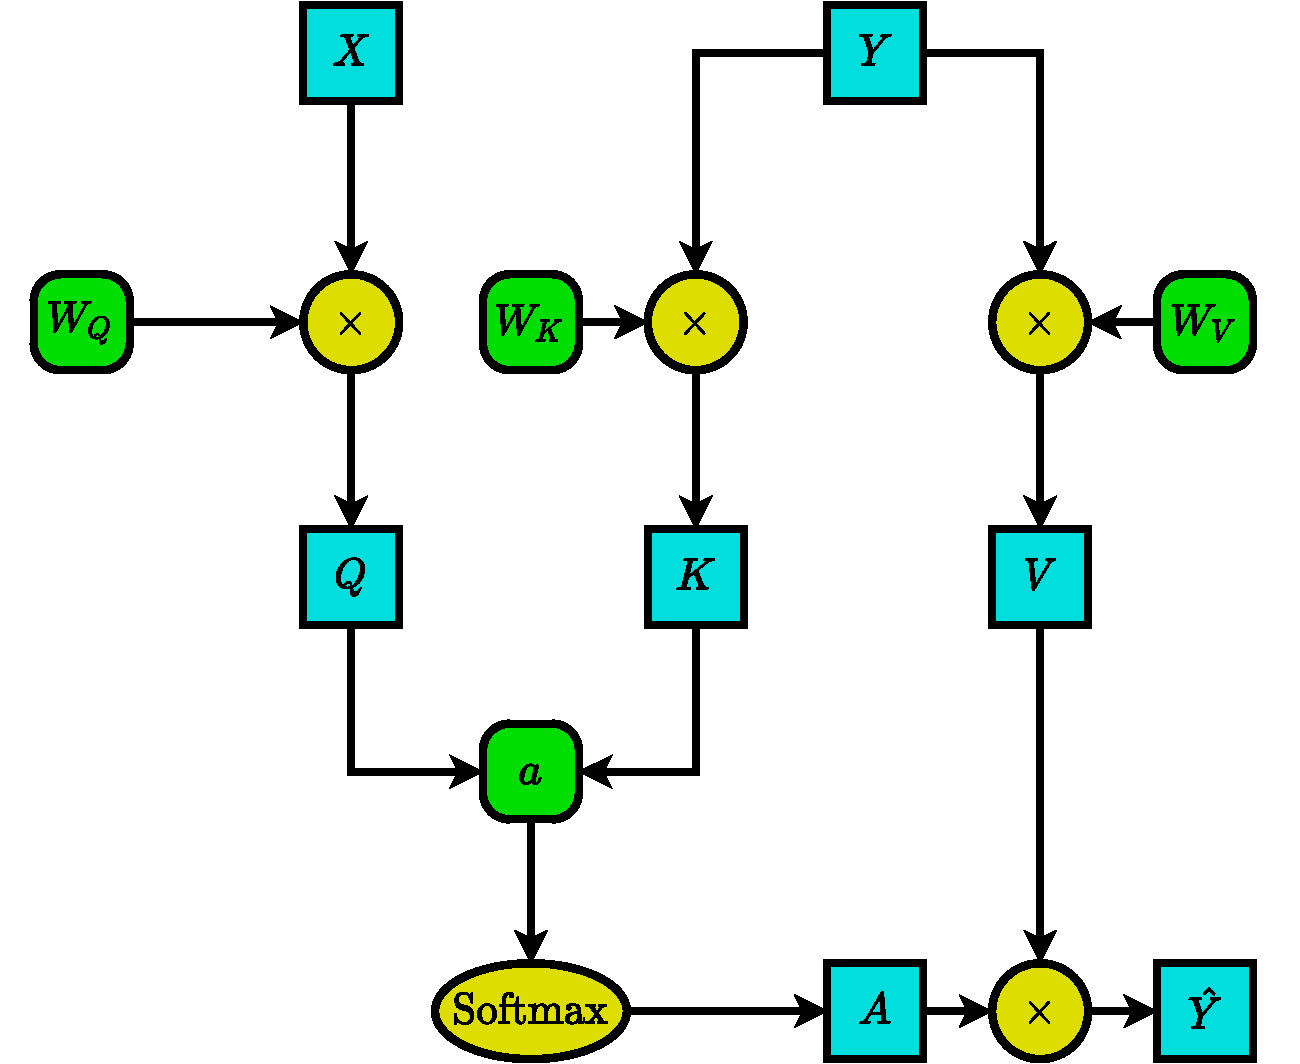
\includegraphics[width=0.5\textwidth]{figures/background/attention.pdf}
\caption[Visualization of a general attention mechanism.]{Visualization of a general attention mechanism.}
\label{fig:attention}
\end{figure}

\subsection{Graph Neural Networks}
Historically, neural network models have seen tremendous success when applied to a highly diverse selection of challenges arising in various scientific disciplines, and graphs are no exception. For more than a decade up until today, research in developing robust neural networks for graph-related tasks has been progressing in parallel with purely graph-embedding-based approaches. However, it is incorrect that these two ideas are disconnected, neural networks for graphs can be generalized beyond the simple single-embedding-layer architecture. Despite the high variety in introduced model design, leading to many model sub-classes, all are usually referred to together with Graph Neural Networks (GNNs).

\cite{battaglia_relational_2018} successfully attempt to aggregate a decade of previous research in graph representation learning using network models into the most general framework that can be used to describe and comprehend the plethora of model designs from a higher-level perspective. 

The authors explain that the general GNN architecture can be viewed as a composition of a finite number of generalized graph processing models, coined GN blocks. Each GN block receives a graph representation as input and outputs a \emph{refined} representation of the graph, such that the representations evolve from the original discrete entity and relation sets into several layers of improvements to some initial embeddings. 

In order to generalize the structure of GN blocks and the operations that need to be performed, the authors allow the generality of the graph definition as well. Graph nodes and edges are allowed to have a whole collection of \emph{attributes} not only single type labels, possibly global attributes attached to the whole graph present as well. For a graph $G=(V, E)$, let $\pmb{v}_i$ denote the attributes of node $v_i \in V$, $\pmb{e}_{ij}$ the attributes of edge $(v_i,v_j)\in E$ and $\pmb{u}$ the global graph attributes. The sequence of operations a general GN block thus has to perform in order to obtain a representation of such rich graphs is visually represented in Figure \ref{fig:general_gn_block} and formally defined below:
\begin{enumerate}
\item Update edge attributes by applying a mapping model per edge: 

$\forall (v_i, v_j) \in E, \pmb{e}'_{ij} = \phi^e(\pmb{e}_{ij},\pmb{v}_i,\pmb{v}_j,\pmb{u})$;
\item Aggregate edge-attributes per node: 

$\forall v_i \in V,\bar{\pmb{e}}'_i = \rho^{e \to v}(E'_i)$, where $E'_i = \{(\pmb{e}'_{ij}, v_i, v_j)| v_j \in V\}$;
\item Update node attributes by applying a mapping model per node: 

$\forall v_i \in V, \pmb{v}'_i = \phi^v(\bar{\pmb{e}}'_i, \pmb{v}_i, \pmb{u})$;
\item Aggregate edge attributes globally: $\bar{\pmb{e}}'=\rho^{e \to u}(E')$, where $E' = \bigcup_{v_i \in V}{E'_i}$;
\item Aggregate node attributes globally: $\bar{\pmb{v}}'=\rho^{v \to u}(V')$, where $V' = \{\pmb{v}'_i| v_i \in V\}$;
\item Update global attributes by applying a mapping model: $\pmb{u}'=\phi^u(\bar{\pmb{e}}', \bar{\pmb{v}}', \pmb{u})$;
\item Output the new graph representation: $G'=(V', E', \pmb{u}')$.
\end{enumerate}

\begin{figure}[H]
\centering
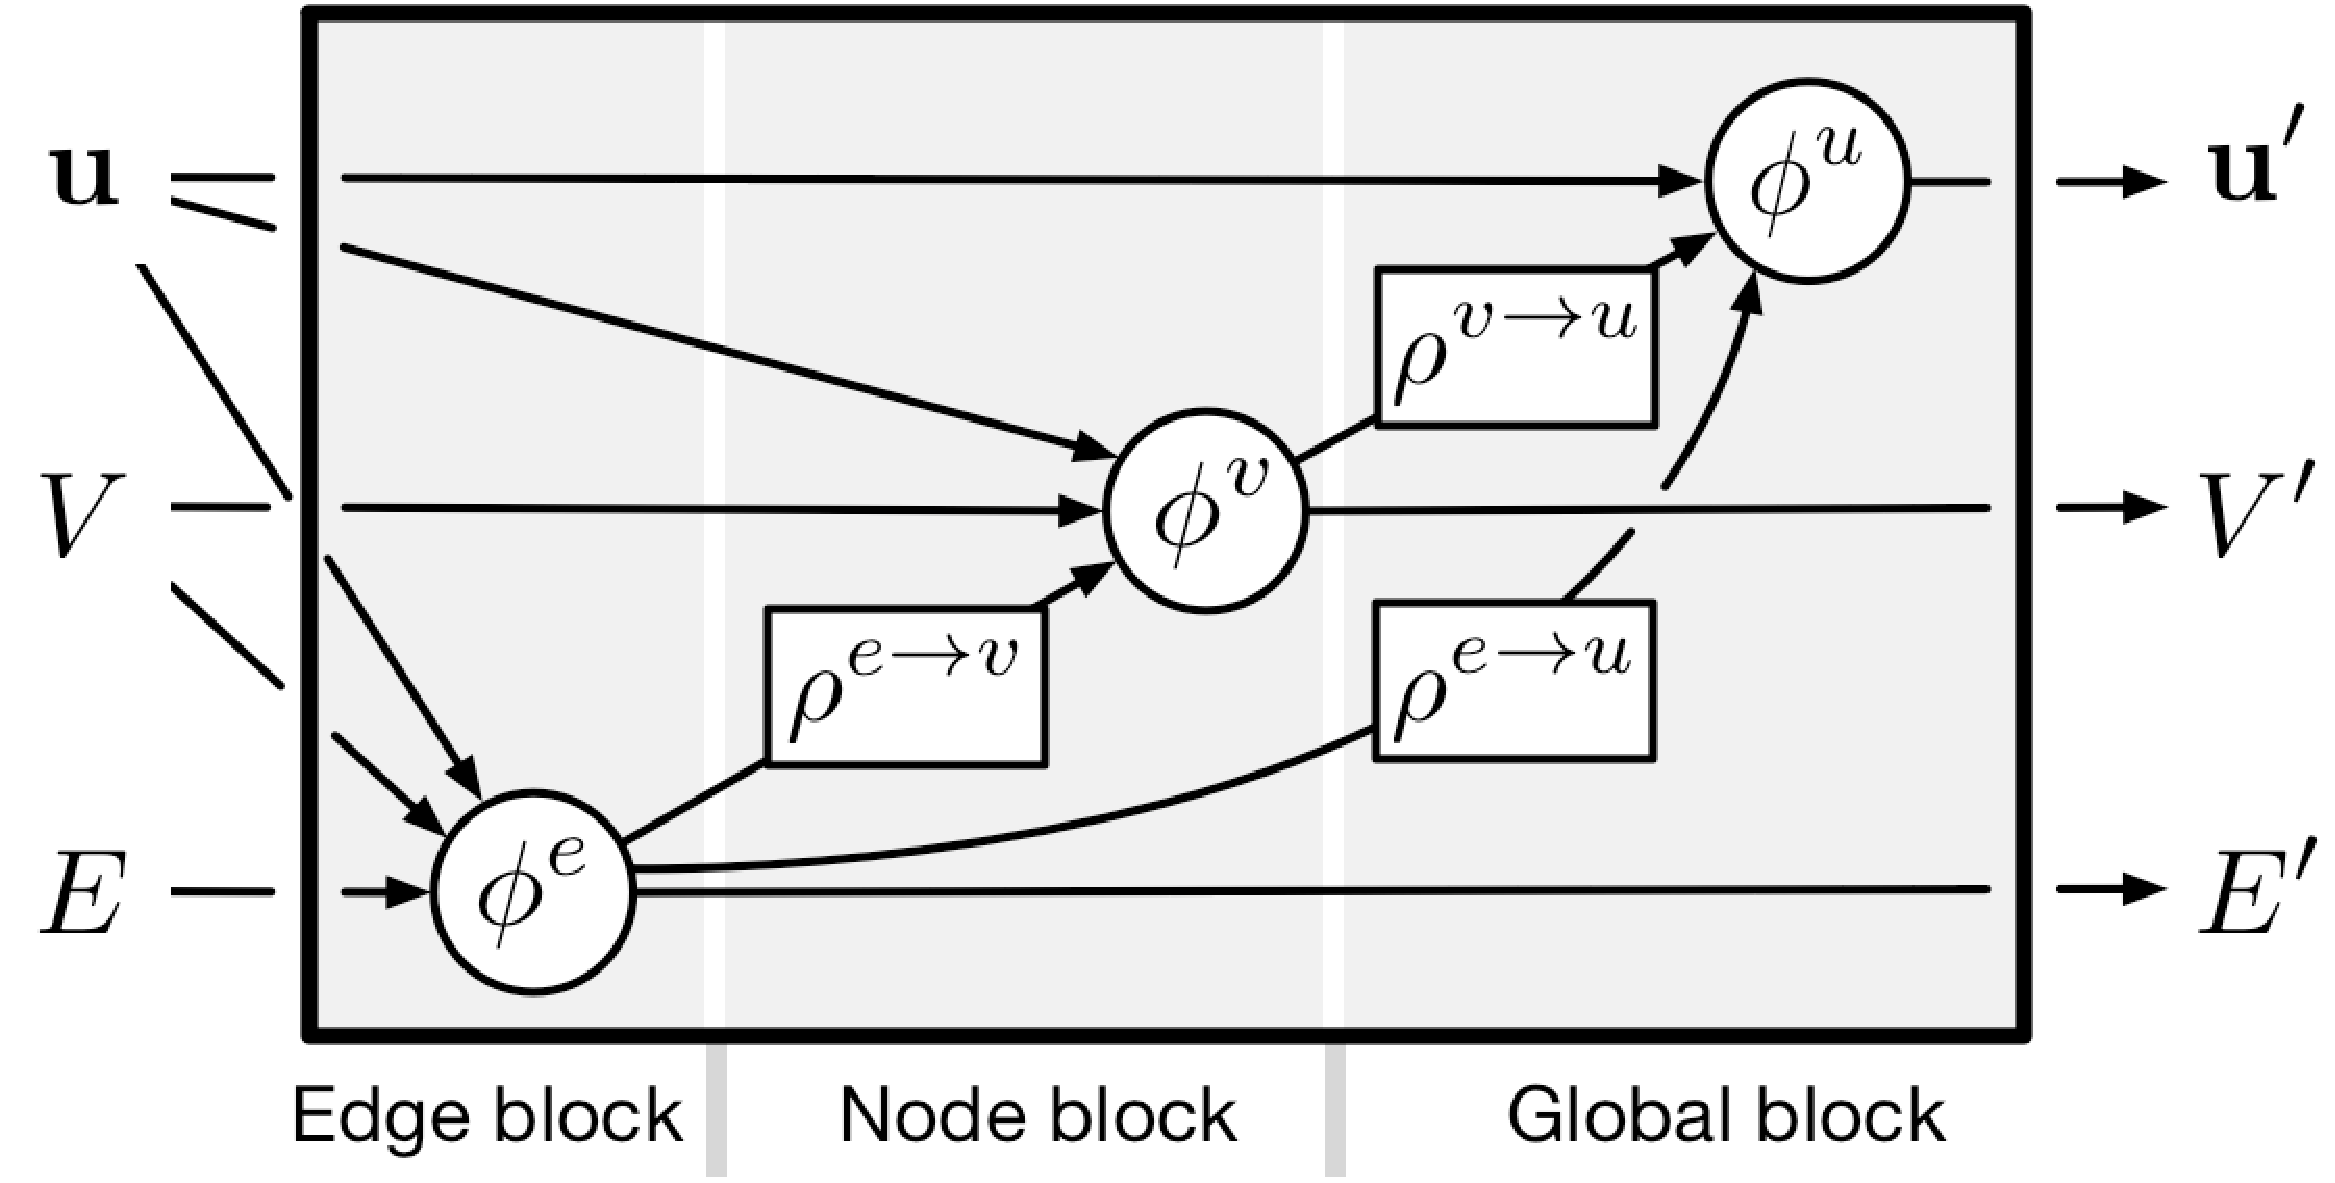
\includegraphics[width=0.75\textwidth]{figures/background/general_gn_block}
\caption[Visualization of the general GN block pipeline.]{Visualization of the general GN block pipeline. \\Courtesy of \cite{battaglia_relational_2018}.}
\label{fig:general_gn_block}
\end{figure}

The mapping models $\phi^e, \phi^v, \phi^u$ can potentially be neural networks of any architecture, while for the aggregation functions $\rho^{e \to v},\rho^{e \to u},\rho^{v \to u}$ usually a mean, sum or max is used.

The proposed framework is helpful in structuring and organizing graph network ideas that can be applied to the most attribute-rich graph.